% Generated by ArticleSignalDiagrams. Opaque vector fills only.
\documentclass[10pt,tikz,border=5pt]{standalone}
\usepackage{lmodern}
\usetikzlibrary{fit}
\begin{document}
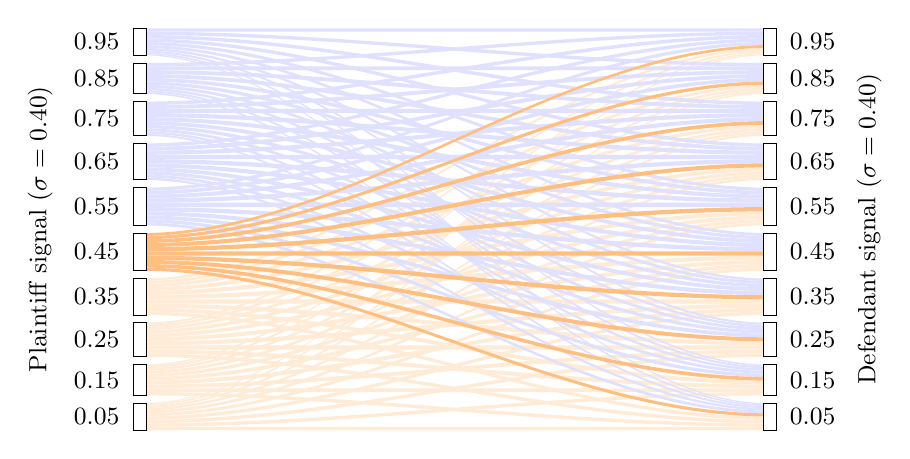
\begin{tikzpicture}[x=1cm,y=1cm,font=\small]\path[fill=orange!16!white,draw=none] (3.3,-5.1) .. controls (6,-5.1) and (8.6,-5.1) .. (11.3,-5.1) -- (11.3,-5.059646) .. controls (8.6,-5.059646) and (6,-5.059646) .. (3.3,-5.059646) -- cycle;
\path[fill=orange!16!white,draw=none] (3.3,-5.059646) .. controls (6,-5.059646) and (8.6,-4.660694) .. (11.3,-4.660694) -- (11.3,-4.617421) .. controls (8.6,-4.617421) and (6,-5.016373) .. (3.3,-5.016373) -- cycle;
\path[fill=orange!16!white,draw=none] (3.3,-5.016373) .. controls (6,-5.016373) and (8.6,-4.170572) .. (11.3,-4.170572) -- (11.3,-4.126371) .. controls (8.6,-4.126371) and (6,-4.972171) .. (3.3,-4.972171) -- cycle;
\path[fill=orange!16!white,draw=none] (3.3,-4.972171) .. controls (6,-4.972171) and (8.6,-3.63862) .. (11.3,-3.63862) -- (11.3,-3.595528) .. controls (8.6,-3.595528) and (6,-4.92908) .. (3.3,-4.92908) -- cycle;
\path[fill=orange!16!white,draw=none] (3.3,-4.92908) .. controls (6,-4.92908) and (8.6,-3.076995) .. (11.3,-3.076995) -- (11.3,-3.036814) .. controls (8.6,-3.036814) and (6,-4.888899) .. (3.3,-4.888899) -- cycle;
\path[fill=orange!16!white,draw=none] (3.3,-4.888899) .. controls (6,-4.888899) and (8.6,-2.5) .. (11.3,-2.5) -- (11.3,-2.464084) .. controls (8.6,-2.464084) and (6,-4.852983) .. (3.3,-4.852983) -- cycle;
\path[fill=orange!16!white,draw=none] (3.3,-4.852983) .. controls (6,-4.852983) and (8.6,-1.923005) .. (11.3,-1.923005) -- (11.3,-1.892163) .. controls (8.6,-1.892163) and (6,-4.822141) .. (3.3,-4.822141) -- cycle;
\path[fill=orange!16!white,draw=none] (3.3,-4.822141) .. controls (6,-4.822141) and (8.6,-1.36138) .. (11.3,-1.36138) -- (11.3,-1.335885) .. controls (8.6,-1.335885) and (6,-4.796646) .. (3.3,-4.796646) -- cycle;
\path[fill=orange!16!white,draw=none] (3.3,-4.796646) .. controls (6,-4.796646) and (8.6,-0.829428) .. (11.3,-0.829428) -- (11.3,-0.809108) .. controls (8.6,-0.809108) and (6,-4.776326) .. (3.3,-4.776326) -- cycle;
\path[fill=orange!16!white,draw=none] (3.3,-4.776326) .. controls (6,-4.776326) and (8.6,-0.339306) .. (11.3,-0.339306) -- (11.3,-0.323674) .. controls (8.6,-0.323674) and (6,-4.760694) .. (3.3,-4.760694) -- cycle;
\path[fill=orange!16!white,draw=none] (3.3,-4.660694) .. controls (6,-4.660694) and (8.6,-5.059646) .. (11.3,-5.059646) -- (11.3,-5.016373) .. controls (8.6,-5.016373) and (6,-4.617421) .. (3.3,-4.617421) -- cycle;
\path[fill=orange!16!white,draw=none] (3.3,-4.617421) .. controls (6,-4.617421) and (8.6,-4.617421) .. (11.3,-4.617421) -- (11.3,-4.570384) .. controls (8.6,-4.570384) and (6,-4.570384) .. (3.3,-4.570384) -- cycle;
\path[fill=orange!16!white,draw=none] (3.3,-4.570384) .. controls (6,-4.570384) and (8.6,-4.126371) .. (11.3,-4.126371) -- (11.3,-4.077573) .. controls (8.6,-4.077573) and (6,-4.521587) .. (3.3,-4.521587) -- cycle;
\path[fill=orange!16!white,draw=none] (3.3,-4.521587) .. controls (6,-4.521587) and (8.6,-3.595528) .. (11.3,-3.595528) -- (11.3,-3.547108) .. controls (8.6,-3.547108) and (6,-4.473166) .. (3.3,-4.473166) -- cycle;
\path[fill=orange!16!white,draw=none] (3.3,-4.473166) .. controls (6,-4.473166) and (8.6,-3.036814) .. (11.3,-3.036814) -- (11.3,-2.990757) .. controls (8.6,-2.990757) and (6,-4.427109) .. (3.3,-4.427109) -- cycle;
\path[fill=orange!16!white,draw=none] (3.3,-4.427109) .. controls (6,-4.427109) and (8.6,-2.464084) .. (11.3,-2.464084) -- (11.3,-2.421997) .. controls (8.6,-2.421997) and (6,-4.385022) .. (3.3,-4.385022) -- cycle;
\path[fill=orange!16!white,draw=none] (3.3,-4.385022) .. controls (6,-4.385022) and (8.6,-1.892163) .. (11.3,-1.892163) -- (11.3,-1.85514) .. controls (8.6,-1.85514) and (6,-4.347999) .. (3.3,-4.347999) -- cycle;
\path[fill=orange!16!white,draw=none] (3.3,-4.347999) .. controls (6,-4.347999) and (8.6,-1.335885) .. (11.3,-1.335885) -- (11.3,-1.304484) .. controls (8.6,-1.304484) and (6,-4.316598) .. (3.3,-4.316598) -- cycle;
\path[fill=orange!16!white,draw=none] (3.3,-4.316598) .. controls (6,-4.316598) and (8.6,-0.809108) .. (11.3,-0.809108) -- (11.3,-0.783402) .. controls (8.6,-0.783402) and (6,-4.290892) .. (3.3,-4.290892) -- cycle;
\path[fill=orange!16!white,draw=none] (3.3,-4.290892) .. controls (6,-4.290892) and (8.6,-0.323674) .. (11.3,-0.323674) -- (11.3,-0.303354) .. controls (8.6,-0.303354) and (6,-4.270572) .. (3.3,-4.270572) -- cycle;
\path[fill=orange!16!white,draw=none] (3.3,-4.170572) .. controls (6,-4.170572) and (8.6,-5.016373) .. (11.3,-5.016373) -- (11.3,-4.972171) .. controls (8.6,-4.972171) and (6,-4.126371) .. (3.3,-4.126371) -- cycle;
\path[fill=orange!16!white,draw=none] (3.3,-4.126371) .. controls (6,-4.126371) and (8.6,-4.570384) .. (11.3,-4.570384) -- (11.3,-4.521587) .. controls (8.6,-4.521587) and (6,-4.077573) .. (3.3,-4.077573) -- cycle;
\path[fill=orange!16!white,draw=none] (3.3,-4.077573) .. controls (6,-4.077573) and (8.6,-4.077573) .. (11.3,-4.077573) -- (11.3,-4.026046) .. controls (8.6,-4.026046) and (6,-4.026046) .. (3.3,-4.026046) -- cycle;
\path[fill=orange!16!white,draw=none] (3.3,-4.026046) .. controls (6,-4.026046) and (8.6,-3.547108) .. (11.3,-3.547108) -- (11.3,-3.494952) .. controls (8.6,-3.494952) and (6,-3.973891) .. (3.3,-3.973891) -- cycle;
\path[fill=orange!16!white,draw=none] (3.3,-3.973891) .. controls (6,-3.973891) and (8.6,-2.990757) .. (11.3,-2.990757) -- (11.3,-2.940039) .. controls (8.6,-2.940039) and (6,-3.923173) .. (3.3,-3.923173) -- cycle;
\path[fill=orange!16!white,draw=none] (3.3,-3.923173) .. controls (6,-3.923173) and (8.6,-2.421997) .. (11.3,-2.421997) -- (11.3,-2.37452) .. controls (8.6,-2.37452) and (6,-3.875697) .. (3.3,-3.875697) -- cycle;
\path[fill=orange!16!white,draw=none] (3.3,-3.875697) .. controls (6,-3.875697) and (8.6,-1.85514) .. (11.3,-1.85514) -- (11.3,-1.81229) .. controls (8.6,-1.81229) and (6,-3.832846) .. (3.3,-3.832846) -- cycle;
\path[fill=orange!16!white,draw=none] (3.3,-3.832846) .. controls (6,-3.832846) and (8.6,-1.304484) .. (11.3,-1.304484) -- (11.3,-1.267154) .. controls (8.6,-1.267154) and (6,-3.795516) .. (3.3,-3.795516) -- cycle;
\path[fill=orange!16!white,draw=none] (3.3,-3.795516) .. controls (6,-3.795516) and (8.6,-0.783402) .. (11.3,-0.783402) -- (11.3,-0.752001) .. controls (8.6,-0.752001) and (6,-3.764115) .. (3.3,-3.764115) -- cycle;
\path[fill=orange!16!white,draw=none] (3.3,-3.764115) .. controls (6,-3.764115) and (8.6,-0.303354) .. (11.3,-0.303354) -- (11.3,-0.277859) .. controls (8.6,-0.277859) and (6,-3.73862) .. (3.3,-3.73862) -- cycle;
\path[fill=orange!16!white,draw=none] (3.3,-3.63862) .. controls (6,-3.63862) and (8.6,-4.972171) .. (11.3,-4.972171) -- (11.3,-4.92908) .. controls (8.6,-4.92908) and (6,-3.595528) .. (3.3,-3.595528) -- cycle;
\path[fill=orange!16!white,draw=none] (3.3,-3.595528) .. controls (6,-3.595528) and (8.6,-4.521587) .. (11.3,-4.521587) -- (11.3,-4.473166) .. controls (8.6,-4.473166) and (6,-3.547108) .. (3.3,-3.547108) -- cycle;
\path[fill=orange!16!white,draw=none] (3.3,-3.547108) .. controls (6,-3.547108) and (8.6,-4.026046) .. (11.3,-4.026046) -- (11.3,-3.973891) .. controls (8.6,-3.973891) and (6,-3.494952) .. (3.3,-3.494952) -- cycle;
\path[fill=orange!16!white,draw=none] (3.3,-3.494952) .. controls (6,-3.494952) and (8.6,-3.494952) .. (11.3,-3.494952) -- (11.3,-3.440981) .. controls (8.6,-3.440981) and (6,-3.440981) .. (3.3,-3.440981) -- cycle;
\path[fill=orange!16!white,draw=none] (3.3,-3.440981) .. controls (6,-3.440981) and (8.6,-2.940039) .. (11.3,-2.940039) -- (11.3,-2.886276) .. controls (8.6,-2.886276) and (6,-3.387218) .. (3.3,-3.387218) -- cycle;
\path[fill=orange!16!white,draw=none] (3.3,-3.387218) .. controls (6,-3.387218) and (8.6,-2.37452) .. (11.3,-2.37452) -- (11.3,-2.322883) .. controls (8.6,-2.322883) and (6,-3.335581) .. (3.3,-3.335581) -- cycle;
\path[fill=orange!16!white,draw=none] (3.3,-3.335581) .. controls (6,-3.335581) and (8.6,-1.81229) .. (11.3,-1.81229) -- (11.3,-1.764419) .. controls (8.6,-1.764419) and (6,-3.28771) .. (3.3,-3.28771) -- cycle;
\path[fill=orange!16!white,draw=none] (3.3,-3.28771) .. controls (6,-3.28771) and (8.6,-1.267154) .. (11.3,-1.267154) -- (11.3,-1.224303) .. controls (8.6,-1.224303) and (6,-3.24486) .. (3.3,-3.24486) -- cycle;
\path[fill=orange!16!white,draw=none] (3.3,-3.24486) .. controls (6,-3.24486) and (8.6,-0.752001) .. (11.3,-0.752001) -- (11.3,-0.714978) .. controls (8.6,-0.714978) and (6,-3.207837) .. (3.3,-3.207837) -- cycle;
\path[fill=orange!16!white,draw=none] (3.3,-3.207837) .. controls (6,-3.207837) and (8.6,-0.277859) .. (11.3,-0.277859) -- (11.3,-0.247017) .. controls (8.6,-0.247017) and (6,-3.176995) .. (3.3,-3.176995) -- cycle;
\path[fill=blue!12!white,draw=none] (3.3,-2.5) .. controls (6,-2.5) and (8.6,-4.888899) .. (11.3,-4.888899) -- (11.3,-4.852983) .. controls (8.6,-4.852983) and (6,-2.464084) .. (3.3,-2.464084) -- cycle;
\path[fill=blue!12!white,draw=none] (3.3,-2.464084) .. controls (6,-2.464084) and (8.6,-4.427109) .. (11.3,-4.427109) -- (11.3,-4.385022) .. controls (8.6,-4.385022) and (6,-2.421997) .. (3.3,-2.421997) -- cycle;
\path[fill=blue!12!white,draw=none] (3.3,-2.421997) .. controls (6,-2.421997) and (8.6,-3.923173) .. (11.3,-3.923173) -- (11.3,-3.875697) .. controls (8.6,-3.875697) and (6,-2.37452) .. (3.3,-2.37452) -- cycle;
\path[fill=blue!12!white,draw=none] (3.3,-2.37452) .. controls (6,-2.37452) and (8.6,-3.387218) .. (11.3,-3.387218) -- (11.3,-3.335581) .. controls (8.6,-3.335581) and (6,-2.322883) .. (3.3,-2.322883) -- cycle;
\path[fill=blue!12!white,draw=none] (3.3,-2.322883) .. controls (6,-2.322883) and (8.6,-2.831326) .. (11.3,-2.831326) -- (11.3,-2.777117) .. controls (8.6,-2.777117) and (6,-2.268674) .. (3.3,-2.268674) -- cycle;
\path[fill=blue!12!white,draw=none] (3.3,-2.268674) .. controls (6,-2.268674) and (8.6,-2.268674) .. (11.3,-2.268674) -- (11.3,-2.213724) .. controls (8.6,-2.213724) and (6,-2.213724) .. (3.3,-2.213724) -- cycle;
\path[fill=blue!12!white,draw=none] (3.3,-2.213724) .. controls (6,-2.213724) and (8.6,-1.712782) .. (11.3,-1.712782) -- (11.3,-1.659019) .. controls (8.6,-1.659019) and (6,-2.159961) .. (3.3,-2.159961) -- cycle;
\path[fill=blue!12!white,draw=none] (3.3,-2.159961) .. controls (6,-2.159961) and (8.6,-1.176827) .. (11.3,-1.176827) -- (11.3,-1.126109) .. controls (8.6,-1.126109) and (6,-2.109243) .. (3.3,-2.109243) -- cycle;
\path[fill=blue!12!white,draw=none] (3.3,-2.109243) .. controls (6,-2.109243) and (8.6,-0.672891) .. (11.3,-0.672891) -- (11.3,-0.626834) .. controls (8.6,-0.626834) and (6,-2.063186) .. (3.3,-2.063186) -- cycle;
\path[fill=blue!12!white,draw=none] (3.3,-2.063186) .. controls (6,-2.063186) and (8.6,-0.211101) .. (11.3,-0.211101) -- (11.3,-0.17092) .. controls (8.6,-0.17092) and (6,-2.023005) .. (3.3,-2.023005) -- cycle;
\path[fill=blue!12!white,draw=none] (3.3,-1.923005) .. controls (6,-1.923005) and (8.6,-4.852983) .. (11.3,-4.852983) -- (11.3,-4.822141) .. controls (8.6,-4.822141) and (6,-1.892163) .. (3.3,-1.892163) -- cycle;
\path[fill=blue!12!white,draw=none] (3.3,-1.892163) .. controls (6,-1.892163) and (8.6,-4.385022) .. (11.3,-4.385022) -- (11.3,-4.347999) .. controls (8.6,-4.347999) and (6,-1.85514) .. (3.3,-1.85514) -- cycle;
\path[fill=blue!12!white,draw=none] (3.3,-1.85514) .. controls (6,-1.85514) and (8.6,-3.875697) .. (11.3,-3.875697) -- (11.3,-3.832846) .. controls (8.6,-3.832846) and (6,-1.81229) .. (3.3,-1.81229) -- cycle;
\path[fill=blue!12!white,draw=none] (3.3,-1.81229) .. controls (6,-1.81229) and (8.6,-3.335581) .. (11.3,-3.335581) -- (11.3,-3.28771) .. controls (8.6,-3.28771) and (6,-1.764419) .. (3.3,-1.764419) -- cycle;
\path[fill=blue!12!white,draw=none] (3.3,-1.764419) .. controls (6,-1.764419) and (8.6,-2.777117) .. (11.3,-2.777117) -- (11.3,-2.72548) .. controls (8.6,-2.72548) and (6,-1.712782) .. (3.3,-1.712782) -- cycle;
\path[fill=blue!12!white,draw=none] (3.3,-1.712782) .. controls (6,-1.712782) and (8.6,-2.213724) .. (11.3,-2.213724) -- (11.3,-2.159961) .. controls (8.6,-2.159961) and (6,-1.659019) .. (3.3,-1.659019) -- cycle;
\path[fill=blue!12!white,draw=none] (3.3,-1.659019) .. controls (6,-1.659019) and (8.6,-1.659019) .. (11.3,-1.659019) -- (11.3,-1.605048) .. controls (8.6,-1.605048) and (6,-1.605048) .. (3.3,-1.605048) -- cycle;
\path[fill=blue!12!white,draw=none] (3.3,-1.605048) .. controls (6,-1.605048) and (8.6,-1.126109) .. (11.3,-1.126109) -- (11.3,-1.073954) .. controls (8.6,-1.073954) and (6,-1.552892) .. (3.3,-1.552892) -- cycle;
\path[fill=blue!12!white,draw=none] (3.3,-1.552892) .. controls (6,-1.552892) and (8.6,-0.626834) .. (11.3,-0.626834) -- (11.3,-0.578413) .. controls (8.6,-0.578413) and (6,-1.504472) .. (3.3,-1.504472) -- cycle;
\path[fill=blue!12!white,draw=none] (3.3,-1.504472) .. controls (6,-1.504472) and (8.6,-0.17092) .. (11.3,-0.17092) -- (11.3,-0.127829) .. controls (8.6,-0.127829) and (6,-1.46138) .. (3.3,-1.46138) -- cycle;
\path[fill=blue!12!white,draw=none] (3.3,-1.36138) .. controls (6,-1.36138) and (8.6,-4.822141) .. (11.3,-4.822141) -- (11.3,-4.796646) .. controls (8.6,-4.796646) and (6,-1.335885) .. (3.3,-1.335885) -- cycle;
\path[fill=blue!12!white,draw=none] (3.3,-1.335885) .. controls (6,-1.335885) and (8.6,-4.347999) .. (11.3,-4.347999) -- (11.3,-4.316598) .. controls (8.6,-4.316598) and (6,-1.304484) .. (3.3,-1.304484) -- cycle;
\path[fill=blue!12!white,draw=none] (3.3,-1.304484) .. controls (6,-1.304484) and (8.6,-3.832846) .. (11.3,-3.832846) -- (11.3,-3.795516) .. controls (8.6,-3.795516) and (6,-1.267154) .. (3.3,-1.267154) -- cycle;
\path[fill=blue!12!white,draw=none] (3.3,-1.267154) .. controls (6,-1.267154) and (8.6,-3.28771) .. (11.3,-3.28771) -- (11.3,-3.24486) .. controls (8.6,-3.24486) and (6,-1.224303) .. (3.3,-1.224303) -- cycle;
\path[fill=blue!12!white,draw=none] (3.3,-1.224303) .. controls (6,-1.224303) and (8.6,-2.72548) .. (11.3,-2.72548) -- (11.3,-2.678003) .. controls (8.6,-2.678003) and (6,-1.176827) .. (3.3,-1.176827) -- cycle;
\path[fill=blue!12!white,draw=none] (3.3,-1.176827) .. controls (6,-1.176827) and (8.6,-2.159961) .. (11.3,-2.159961) -- (11.3,-2.109243) .. controls (8.6,-2.109243) and (6,-1.126109) .. (3.3,-1.126109) -- cycle;
\path[fill=blue!12!white,draw=none] (3.3,-1.126109) .. controls (6,-1.126109) and (8.6,-1.605048) .. (11.3,-1.605048) -- (11.3,-1.552892) .. controls (8.6,-1.552892) and (6,-1.073954) .. (3.3,-1.073954) -- cycle;
\path[fill=blue!12!white,draw=none] (3.3,-1.073954) .. controls (6,-1.073954) and (8.6,-1.073954) .. (11.3,-1.073954) -- (11.3,-1.022427) .. controls (8.6,-1.022427) and (6,-1.022427) .. (3.3,-1.022427) -- cycle;
\path[fill=blue!12!white,draw=none] (3.3,-1.022427) .. controls (6,-1.022427) and (8.6,-0.578413) .. (11.3,-0.578413) -- (11.3,-0.529616) .. controls (8.6,-0.529616) and (6,-0.973629) .. (3.3,-0.973629) -- cycle;
\path[fill=blue!12!white,draw=none] (3.3,-0.973629) .. controls (6,-0.973629) and (8.6,-0.127829) .. (11.3,-0.127829) -- (11.3,-0.083627) .. controls (8.6,-0.083627) and (6,-0.929428) .. (3.3,-0.929428) -- cycle;
\path[fill=blue!12!white,draw=none] (3.3,-0.829428) .. controls (6,-0.829428) and (8.6,-4.796646) .. (11.3,-4.796646) -- (11.3,-4.776326) .. controls (8.6,-4.776326) and (6,-0.809108) .. (3.3,-0.809108) -- cycle;
\path[fill=blue!12!white,draw=none] (3.3,-0.809108) .. controls (6,-0.809108) and (8.6,-4.316598) .. (11.3,-4.316598) -- (11.3,-4.290892) .. controls (8.6,-4.290892) and (6,-0.783402) .. (3.3,-0.783402) -- cycle;
\path[fill=blue!12!white,draw=none] (3.3,-0.783402) .. controls (6,-0.783402) and (8.6,-3.795516) .. (11.3,-3.795516) -- (11.3,-3.764115) .. controls (8.6,-3.764115) and (6,-0.752001) .. (3.3,-0.752001) -- cycle;
\path[fill=blue!12!white,draw=none] (3.3,-0.752001) .. controls (6,-0.752001) and (8.6,-3.24486) .. (11.3,-3.24486) -- (11.3,-3.207837) .. controls (8.6,-3.207837) and (6,-0.714978) .. (3.3,-0.714978) -- cycle;
\path[fill=blue!12!white,draw=none] (3.3,-0.714978) .. controls (6,-0.714978) and (8.6,-2.678003) .. (11.3,-2.678003) -- (11.3,-2.635916) .. controls (8.6,-2.635916) and (6,-0.672891) .. (3.3,-0.672891) -- cycle;
\path[fill=blue!12!white,draw=none] (3.3,-0.672891) .. controls (6,-0.672891) and (8.6,-2.109243) .. (11.3,-2.109243) -- (11.3,-2.063186) .. controls (8.6,-2.063186) and (6,-0.626834) .. (3.3,-0.626834) -- cycle;
\path[fill=blue!12!white,draw=none] (3.3,-0.626834) .. controls (6,-0.626834) and (8.6,-1.552892) .. (11.3,-1.552892) -- (11.3,-1.504472) .. controls (8.6,-1.504472) and (6,-0.578413) .. (3.3,-0.578413) -- cycle;
\path[fill=blue!12!white,draw=none] (3.3,-0.578413) .. controls (6,-0.578413) and (8.6,-1.022427) .. (11.3,-1.022427) -- (11.3,-0.973629) .. controls (8.6,-0.973629) and (6,-0.529616) .. (3.3,-0.529616) -- cycle;
\path[fill=blue!12!white,draw=none] (3.3,-0.529616) .. controls (6,-0.529616) and (8.6,-0.529616) .. (11.3,-0.529616) -- (11.3,-0.482579) .. controls (8.6,-0.482579) and (6,-0.482579) .. (3.3,-0.482579) -- cycle;
\path[fill=blue!12!white,draw=none] (3.3,-0.482579) .. controls (6,-0.482579) and (8.6,-0.083627) .. (11.3,-0.083627) -- (11.3,-0.040354) .. controls (8.6,-0.040354) and (6,-0.439306) .. (3.3,-0.439306) -- cycle;
\path[fill=blue!12!white,draw=none] (3.3,-0.339306) .. controls (6,-0.339306) and (8.6,-4.776326) .. (11.3,-4.776326) -- (11.3,-4.760694) .. controls (8.6,-4.760694) and (6,-0.323674) .. (3.3,-0.323674) -- cycle;
\path[fill=blue!12!white,draw=none] (3.3,-0.323674) .. controls (6,-0.323674) and (8.6,-4.290892) .. (11.3,-4.290892) -- (11.3,-4.270572) .. controls (8.6,-4.270572) and (6,-0.303354) .. (3.3,-0.303354) -- cycle;
\path[fill=blue!12!white,draw=none] (3.3,-0.303354) .. controls (6,-0.303354) and (8.6,-3.764115) .. (11.3,-3.764115) -- (11.3,-3.73862) .. controls (8.6,-3.73862) and (6,-0.277859) .. (3.3,-0.277859) -- cycle;
\path[fill=blue!12!white,draw=none] (3.3,-0.277859) .. controls (6,-0.277859) and (8.6,-3.207837) .. (11.3,-3.207837) -- (11.3,-3.176995) .. controls (8.6,-3.176995) and (6,-0.247017) .. (3.3,-0.247017) -- cycle;
\path[fill=blue!12!white,draw=none] (3.3,-0.247017) .. controls (6,-0.247017) and (8.6,-2.635916) .. (11.3,-2.635916) -- (11.3,-2.6) .. controls (8.6,-2.6) and (6,-0.211101) .. (3.3,-0.211101) -- cycle;
\path[fill=blue!12!white,draw=none] (3.3,-0.211101) .. controls (6,-0.211101) and (8.6,-2.063186) .. (11.3,-2.063186) -- (11.3,-2.023005) .. controls (8.6,-2.023005) and (6,-0.17092) .. (3.3,-0.17092) -- cycle;
\path[fill=blue!12!white,draw=none] (3.3,-0.17092) .. controls (6,-0.17092) and (8.6,-1.504472) .. (11.3,-1.504472) -- (11.3,-1.46138) .. controls (8.6,-1.46138) and (6,-0.127829) .. (3.3,-0.127829) -- cycle;
\path[fill=blue!12!white,draw=none] (3.3,-0.127829) .. controls (6,-0.127829) and (8.6,-0.973629) .. (11.3,-0.973629) -- (11.3,-0.929428) .. controls (8.6,-0.929428) and (6,-0.083627) .. (3.3,-0.083627) -- cycle;
\path[fill=blue!12!white,draw=none] (3.3,-0.083627) .. controls (6,-0.083627) and (8.6,-0.482579) .. (11.3,-0.482579) -- (11.3,-0.439306) .. controls (8.6,-0.439306) and (6,-0.040354) .. (3.3,-0.040354) -- cycle;
\path[fill=blue!12!white,draw=none] (3.3,-0.040354) .. controls (6,-0.040354) and (8.6,-0.040354) .. (11.3,-0.040354) -- (11.3,0) .. controls (8.6,0) and (6,0) .. (3.3,0) -- cycle;
\path[fill=orange!50!white,draw=none] (3.3,-3.076995) .. controls (6,-3.076995) and (8.6,-4.92908) .. (11.3,-4.92908) -- (11.3,-4.888899) .. controls (8.6,-4.888899) and (6,-3.036814) .. (3.3,-3.036814) -- cycle;
\path[fill=orange!50!white,draw=none] (3.3,-3.036814) .. controls (6,-3.036814) and (8.6,-4.473166) .. (11.3,-4.473166) -- (11.3,-4.427109) .. controls (8.6,-4.427109) and (6,-2.990757) .. (3.3,-2.990757) -- cycle;
\path[fill=orange!50!white,draw=none] (3.3,-2.990757) .. controls (6,-2.990757) and (8.6,-3.973891) .. (11.3,-3.973891) -- (11.3,-3.923173) .. controls (8.6,-3.923173) and (6,-2.940039) .. (3.3,-2.940039) -- cycle;
\path[fill=orange!50!white,draw=none] (3.3,-2.940039) .. controls (6,-2.940039) and (8.6,-3.440981) .. (11.3,-3.440981) -- (11.3,-3.387218) .. controls (8.6,-3.387218) and (6,-2.886276) .. (3.3,-2.886276) -- cycle;
\path[fill=orange!50!white,draw=none] (3.3,-2.886276) .. controls (6,-2.886276) and (8.6,-2.886276) .. (11.3,-2.886276) -- (11.3,-2.831326) .. controls (8.6,-2.831326) and (6,-2.831326) .. (3.3,-2.831326) -- cycle;
\path[fill=orange!50!white,draw=none] (3.3,-2.831326) .. controls (6,-2.831326) and (8.6,-2.322883) .. (11.3,-2.322883) -- (11.3,-2.268674) .. controls (8.6,-2.268674) and (6,-2.777117) .. (3.3,-2.777117) -- cycle;
\path[fill=orange!50!white,draw=none] (3.3,-2.777117) .. controls (6,-2.777117) and (8.6,-1.764419) .. (11.3,-1.764419) -- (11.3,-1.712782) .. controls (8.6,-1.712782) and (6,-2.72548) .. (3.3,-2.72548) -- cycle;
\path[fill=orange!50!white,draw=none] (3.3,-2.72548) .. controls (6,-2.72548) and (8.6,-1.224303) .. (11.3,-1.224303) -- (11.3,-1.176827) .. controls (8.6,-1.176827) and (6,-2.678003) .. (3.3,-2.678003) -- cycle;
\path[fill=orange!50!white,draw=none] (3.3,-2.678003) .. controls (6,-2.678003) and (8.6,-0.714978) .. (11.3,-0.714978) -- (11.3,-0.672891) .. controls (8.6,-0.672891) and (6,-2.635916) .. (3.3,-2.635916) -- cycle;
\path[fill=orange!50!white,draw=none] (3.3,-2.635916) .. controls (6,-2.635916) and (8.6,-0.247017) .. (11.3,-0.247017) -- (11.3,-0.211101) .. controls (8.6,-0.211101) and (6,-2.6) .. (3.3,-2.6) -- cycle;
\coordinate (axis-midline-0) at (0,-2.55);
\path[fill=white,draw=black,line width=0.3pt] (3.22,-5.1) rectangle (3.38,-4.760694);
\node[anchor=east,fill=white,inner sep=2pt] (bucket-0-0-0) at (3.12,-4.930347) {0.05};
\path[fill=white,draw=black,line width=0.3pt] (3.22,-4.660694) rectangle (3.38,-4.270572);
\node[anchor=east,fill=white,inner sep=2pt] (bucket-0-0-1) at (3.12,-4.465633) {0.15};
\path[fill=white,draw=black,line width=0.3pt] (3.22,-4.170572) rectangle (3.38,-3.73862);
\node[anchor=east,fill=white,inner sep=2pt] (bucket-0-0-2) at (3.12,-3.954596) {0.25};
\path[fill=white,draw=black,line width=0.3pt] (3.22,-3.63862) rectangle (3.38,-3.176995);
\node[anchor=east,fill=white,inner sep=2pt] (bucket-0-0-3) at (3.12,-3.407808) {0.35};
\path[fill=white,draw=black,line width=0.3pt] (3.22,-3.076995) rectangle (3.38,-2.6);
\node[anchor=east,fill=white,inner sep=2pt] (bucket-0-0-4) at (3.12,-2.838498) {0.45};
\path[fill=white,draw=black,line width=0.3pt] (3.22,-2.5) rectangle (3.38,-2.023005);
\node[anchor=east,fill=white,inner sep=2pt] (bucket-0-0-5) at (3.12,-2.261502) {0.55};
\path[fill=white,draw=black,line width=0.3pt] (3.22,-1.923005) rectangle (3.38,-1.46138);
\node[anchor=east,fill=white,inner sep=2pt] (bucket-0-0-6) at (3.12,-1.692192) {0.65};
\path[fill=white,draw=black,line width=0.3pt] (3.22,-1.36138) rectangle (3.38,-0.929428);
\node[anchor=east,fill=white,inner sep=2pt] (bucket-0-0-7) at (3.12,-1.145404) {0.75};
\path[fill=white,draw=black,line width=0.3pt] (3.22,-0.829428) rectangle (3.38,-0.439306);
\node[anchor=east,fill=white,inner sep=2pt] (bucket-0-0-8) at (3.12,-0.634367) {0.85};
\path[fill=white,draw=black,line width=0.3pt] (3.22,-0.339306) rectangle (3.38,0);
\node[anchor=east,fill=white,inner sep=2pt] (bucket-0-0-9) at (3.12,-0.169653) {0.95};
\node[fit=(bucket-0-0-0) (bucket-0-0-1) (bucket-0-0-2) (bucket-0-0-3) (bucket-0-0-4) (bucket-0-0-5) (bucket-0-0-6) (bucket-0-0-7) (bucket-0-0-8) (bucket-0-0-9),inner sep=0pt] (source-labels-0) {};
\coordinate (axis-title-0-0) at (source-labels-0.west |- axis-midline-0);
\node[rotate=90,anchor=south,inner sep=0pt] at ([xshift=-0.18cm]axis-title-0-0) {Plaintiff signal ($\sigma=0.40$)};
\path[fill=white,draw=black,line width=0.3pt] (11.22,-5.1) rectangle (11.38,-4.760694);
\node[anchor=west,fill=white,inner sep=2pt] (bucket-0-1-0) at (11.48,-4.930347) {0.05};
\path[fill=white,draw=black,line width=0.3pt] (11.22,-4.660694) rectangle (11.38,-4.270572);
\node[anchor=west,fill=white,inner sep=2pt] (bucket-0-1-1) at (11.48,-4.465633) {0.15};
\path[fill=white,draw=black,line width=0.3pt] (11.22,-4.170572) rectangle (11.38,-3.73862);
\node[anchor=west,fill=white,inner sep=2pt] (bucket-0-1-2) at (11.48,-3.954596) {0.25};
\path[fill=white,draw=black,line width=0.3pt] (11.22,-3.63862) rectangle (11.38,-3.176995);
\node[anchor=west,fill=white,inner sep=2pt] (bucket-0-1-3) at (11.48,-3.407808) {0.35};
\path[fill=white,draw=black,line width=0.3pt] (11.22,-3.076995) rectangle (11.38,-2.6);
\node[anchor=west,fill=white,inner sep=2pt] (bucket-0-1-4) at (11.48,-2.838498) {0.45};
\path[fill=white,draw=black,line width=0.3pt] (11.22,-2.5) rectangle (11.38,-2.023005);
\node[anchor=west,fill=white,inner sep=2pt] (bucket-0-1-5) at (11.48,-2.261502) {0.55};
\path[fill=white,draw=black,line width=0.3pt] (11.22,-1.923005) rectangle (11.38,-1.46138);
\node[anchor=west,fill=white,inner sep=2pt] (bucket-0-1-6) at (11.48,-1.692192) {0.65};
\path[fill=white,draw=black,line width=0.3pt] (11.22,-1.36138) rectangle (11.38,-0.929428);
\node[anchor=west,fill=white,inner sep=2pt] (bucket-0-1-7) at (11.48,-1.145404) {0.75};
\path[fill=white,draw=black,line width=0.3pt] (11.22,-0.829428) rectangle (11.38,-0.439306);
\node[anchor=west,fill=white,inner sep=2pt] (bucket-0-1-8) at (11.48,-0.634367) {0.85};
\path[fill=white,draw=black,line width=0.3pt] (11.22,-0.339306) rectangle (11.38,0);
\node[anchor=west,fill=white,inner sep=2pt] (bucket-0-1-9) at (11.48,-0.169653) {0.95};
\node[fit=(bucket-0-1-0) (bucket-0-1-1) (bucket-0-1-2) (bucket-0-1-3) (bucket-0-1-4) (bucket-0-1-5) (bucket-0-1-6) (bucket-0-1-7) (bucket-0-1-8) (bucket-0-1-9),inner sep=0pt] (destination-labels-0) {};
\coordinate (axis-title-0-1) at (destination-labels-0.east |- axis-midline-0);
\node[rotate=90,anchor=north,inner sep=0pt] at ([xshift=0.18cm]axis-title-0-1) {Defendant signal ($\sigma=0.40$)};
\end{tikzpicture}
\end{document}

